\documentclass[a4paper,11pt]{article}

%---Packages utilisés
\usepackage[utf8]{inputenc}
\usepackage[T1]{fontenc}
\usepackage[frenchb]{babel}
\usepackage{indentfirst}
\usepackage[]{graphicx}
\usepackage{amsmath}
\usepackage{ccaption}
\usepackage{vmargin}
\usepackage{textcomp}
\usepackage{fancyhdr}
%\usepackage[avantgarde]{quotchap}
\usepackage[Lenny]{fncychap}
\usepackage{cite}
\usepackage{siunitx}

\fancypagestyle{plain}{
\fancyhead[]{}
\fancyfoot[R]{\thepage}
\renewcommand{\headrulewidth}{0pt}}

%---Nouvelles commandes
\newcommand{\arronax}{\textsc{Arronax}}
\newcommand{\cyrce}{\textsc{Cyrcé}}
\newcommand{\Root}{\textsc{Root}}
\renewcommand{\baselinestretch}{1.2}

%\renewcommand{\chaptermark}[1]{%
% \markboth{\thechapter . \ #1}{}}

%---Mise en page
\setlength{\parindent}{2ex}
%\pagestyle{fancy}

%---Début du document
\begin{document}

%---Marges du document
\setmarginsrb{3.5cm}{1.5cm}{1.5cm}{2cm}{2ex}{3ex}{2ex}{5ex}
%1 est la marge gauche
%2 est la marge en haut
%3 est la marge droite 
%4 est la marge en bas
%5 fixe la hauteur de l'etête
%6 fixe la distance entre l'entte et le texte
%7 fixe la hauteur du pied de page
%8 fixe la distance entre le texte et le pied de page
%
%\chapterstyle{veelo}
%\renewcommand{\sectionmark}[1]{\markright{\thesection\ #1}}
\lhead[]{}
\fancyfoot[C]{}
\fancyfoot[R]{\thepage}

%%%%%%%%%%%%%%%%
\begin{center}
\subsection*{Mesures des impédances d'entrée des électromètres}
\end{center}

Avant de procéder à la création d'un système de division de courant pour l'électronique Faster de Dosion, il convient de connaître les impédances d'entrée $R$ des électromètres.
Pour cela nous utilisons un pont diviseur, connecté à une seule piste d'électromètre, et alimenté par une pile AA de 1.5 V, figure \ref{fig:manip}.

\begin{figure}[h]
\begin{center}
\begin{minipage}[c]{0.48\linewidth}
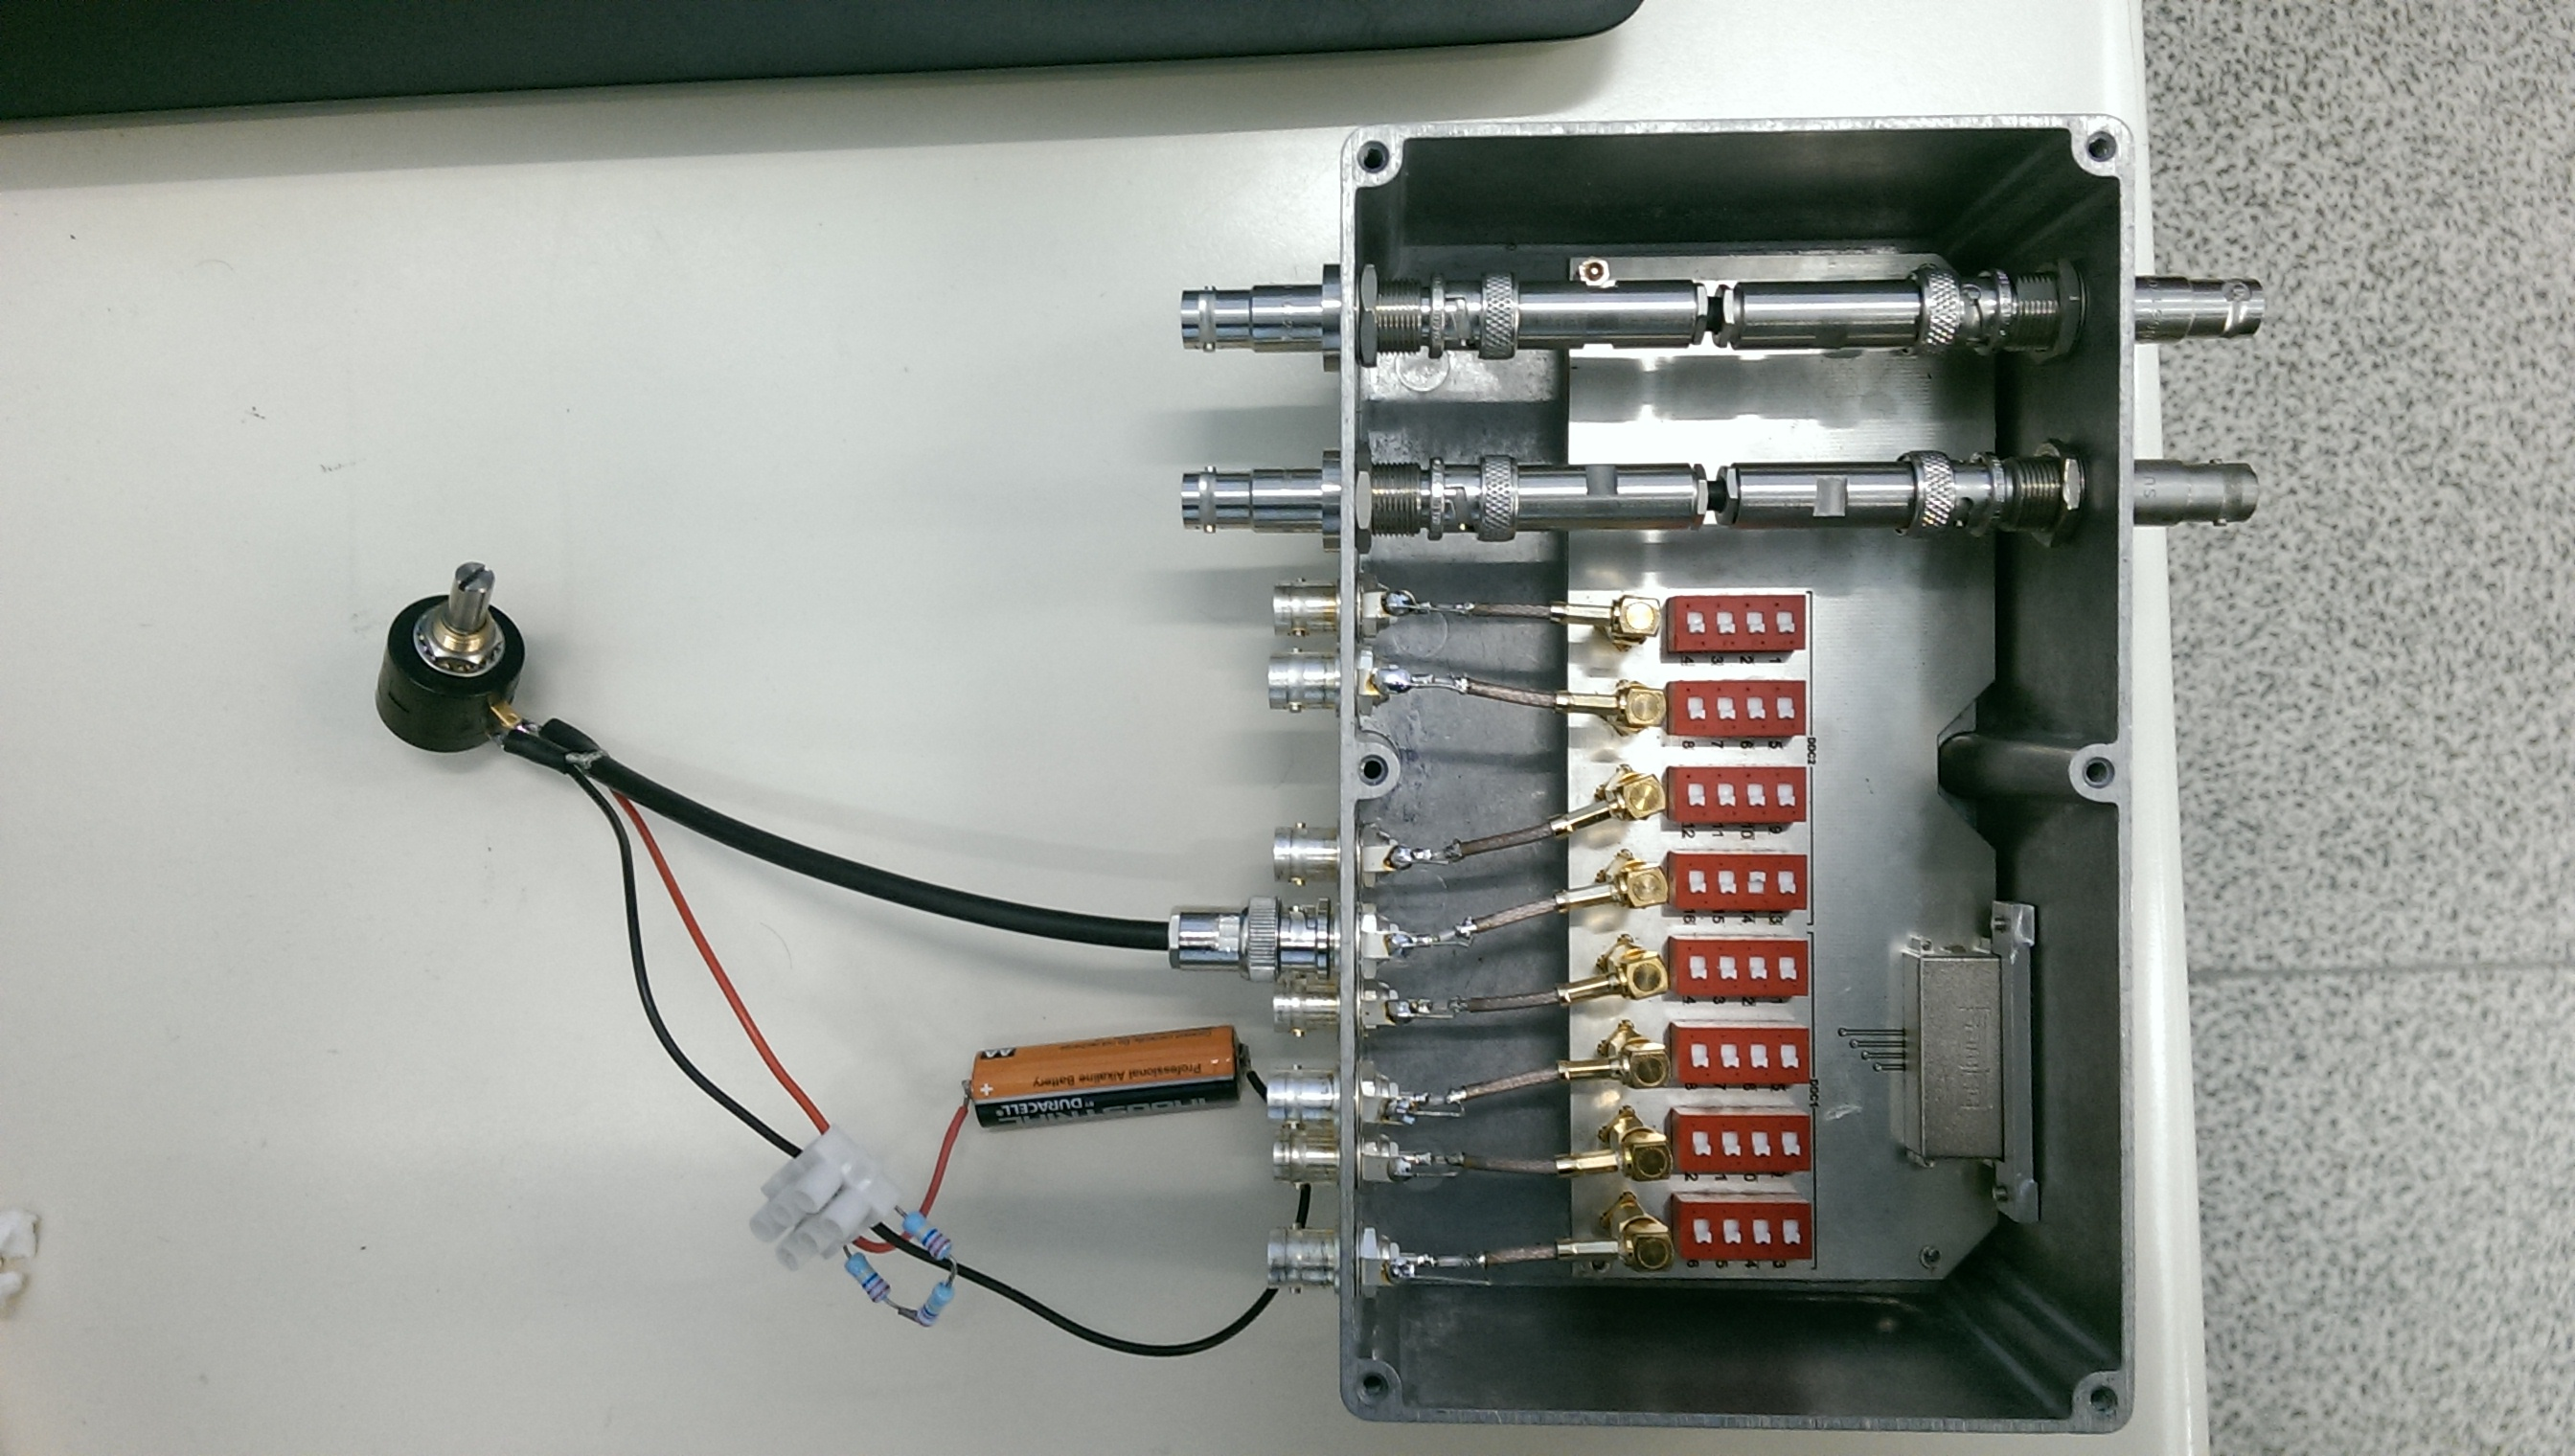
\includegraphics[width=\linewidth]{Montage_photo.jpg} 
\end{minipage}
\hfill
\begin{minipage}[c]{0.48\linewidth}
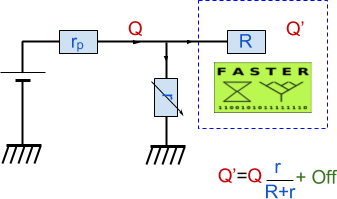
\includegraphics[width=\linewidth]{Montage_schema.png} 
\end{minipage}
\caption{\label{fig:manip}\footnotesize{Photo et schéma du dispositif de mesure}}
\end{center}
\end{figure}
Un potentiomètre de 50 k$\Omega$ est utilisé pour faire varier $r$ et ainsi permettre la détermination du courant offset $Off$ et donc de l'impédance $R$ .

\subsubsection*{Temps d'intégration de 20 $\mu$s}
La valeur de l'impédance d'entrée variant suivant le temps d'intégration défini sur les électromètres , une première mesure est effectuée pour la valeur minimale de 20 $\mu$s. Nous réglons Faster pour qu'il considère 1200 intégrations soit un temps total de 24 ms.

La limite des électromètres est de 12 pC pour une intégration, ce qui dans ce cas donne un courant supporté maximal de : 
$$\frac{12\ \text{ pC}}{20\ \mu\text{s}}=600\ \text{nA}$$
La pile elle délivre une tension de 1.56 V, en plaçant une résistance $r_p$ de 100 M$\Omega$ nous limiterons le courant à :
$$\frac{1.56\ \text{ V}}{100\ \text{M}\Omega}=15.6\ \text{nA}$$
Ce qui est bien inférieur à la limite des électromètres.

Pour contrôler si nous retrouvons bien ce que nous sommes en droit d'attendre, nous avons effectué une première mesure en dessoudant une patte du potentiomètre, et ainsi simulé une résistance $r$ infinie, \textit{i.e} $Q'=Q+Off$, avec :
$$Q=15.6\text{ nA}\times 20\ \mu\text{s}\times 1200$$
$$Q=374.4\text{ pC}$$
Dans ce cas là, la valeur de $Off$ est celle obtenue en l'absence de signal, elle vaut environ $250$ pC, nous devrions obtenir une valeur $Q' \approx\ 625$ pC, et c'est bien ce que nous observons.

Plusieurs mesures de $Q'$ sont donc réalisées avec des valeurs de $r$ différentes et relevées à chaque fois.
La valeur de $Off$ étant différente de celle sans dérivation, car l'entrée dans ce cas est raccordée à une masse par l'intermédiaire de cette dérivation, nous sommes bien face à une équation de 3 inconnues : $Q$, $R$ et $Off$.
Nous obtenons 4 jeux de valeurs :
\begin{center}
\begin{tabular}{llcl}
\multicolumn{4}{c}{$Q'_i=Q\dfrac{r_i}{R+r_i}+Off$}\\
&&&\\
$i=1$:&$r_1=49.5\text{ k}\Omega$&$\Rightarrow$&$Q_1=590\text{ pC}$\\
$i=2$:&$r_2=10.4\text{ k}\Omega$&$\Rightarrow$&$Q_2=462\text{ pC}$\\
$i=3$:&$r_3=2.25\text{ k}\Omega$&$\Rightarrow$&$Q_3=300\text{ pC}$\\
$i=4$:&$r_4=25\ \Omega$&$\Rightarrow$&$Q_4=192\text{ pC}$\\
\end{tabular}
\end{center}

La dernière mesure pour laquelle on assume que $R\gg r$ nous donne la valeur de l'offset :
$$Off=192\text{ pC}$$

Un réarrangement des équations nous donne :
$$R=\frac{r_jr_i(1-A)}{Ar_i-r_j}$$
avec :
$$A=\frac{Q'_j-Off}{Q'_i-Off}$$

Les résolutions de cette équation nous donne :
\begin{center}
\begin{tabular}{lr}
$i=1; j=2$:&$R=7.14\text{ k}\Omega$\\
$i=1; j=3$:&$R=7.26\text{ k}\Omega$\\
$i=2; j=3$:&$R=7.35\text{ k}\Omega$\\
\end{tabular}
\end{center}

Une autre série de mesures réalisée sur un autre électromètre, avec un réglage de 120 intégrations nous donne les valeurs suivantes :
\begin{center}
\begin{tabular}{llcl}
$i=1$:&$r_1=49.4\text{ k}\Omega$&$\Rightarrow$&$Q_1=58\text{ pC}$\\
$i=2$:&$r_2=6.28\text{ k}\Omega$&$\Rightarrow$&$Q_2=40\text{ pC}$\\
$i=3$:&$r_3=22.5\Omega$&$\Rightarrow$&$Q_3=17\text{ pC}$\\
\end{tabular}
\end{center}
La résolution nous amène à cette valeur de $R$ :
\begin{center}
\begin{tabular}{lr}
$i=1; j=2$:&$R=6.35\text{ k}\Omega$\\
\end{tabular}
\end{center}

Bien qu'effectuée sur un électromètre différent, la valeur de l'impédance interne reste dans la même gamme de valeurs.

\subsubsection*{Temps d'intégration de 500 $\mu$s}
Une dernière série de mesures, pour un temps d'intégration différent, un paramètre faisant évoluer l'impédance d'entrée, a été réalisée.
La limite étant toujours de 12 pC par intégration, le courant maximum est dans ce cas de 24 nA, ce qui est toujours supérieur aux 15.6 nA délivrés par la pile.

Les valeurs suivantes sont obtenues :
\begin{center}
\begin{tabular}{llcl}
$i=1$:&$r_1=50.7\text{ k}\Omega$&$\Rightarrow$&$Q_1=800\text{ pC}$\\
$i=2$:&$r_2=8.89\text{ k}\Omega$&$\Rightarrow$&$Q_2=410\text{ pC}$\\
$i=3$:&$r_3=11.72\text{ k}\Omega$&$\Rightarrow$&$Q_3=500\text{ pC}$\\
$i=4$:&$r_4=22.4\ \Omega$&$\Rightarrow$&$Q_4=3.5\text{ pC}$\\
\end{tabular}
\end{center}

De manière identique nous arrivons aux résultats :
\begin{center}
\begin{tabular}{llcl}
$i=1; j=2$:&$R=13.0\text{ k}\Omega$\\
$i=1; j=3$:&$R=11.26\text{ k}\Omega$\\
$i=2; j=3$:&$R=11.89\text{ k}\Omega$\\
\end{tabular}
\end{center}

La valeur de l'impédance est donc différente et supérieure à celle pour des temps d'intégration de 20 $\mu$s, ce qui s'explique par le fonctionnement même des électromètres. Dans tous les cas, nous conservons le même ordre de grandeur de la dizaine de kilo-ohms. 

%%%%%%%%%%%%%%%%%%%%%%%%%%%%%%%%%%

\end{document}

%%%%%%%%%%%%%%%%%%%%%%%%%%%%%%%%%%%%%%%%%%%%%%%%%%%%%%%%%%%%%%%%%%%%%%%%%%%%%%%%%%%%%%%%%%%%%%%%%%